\usetikzlibrary{arrows.meta}
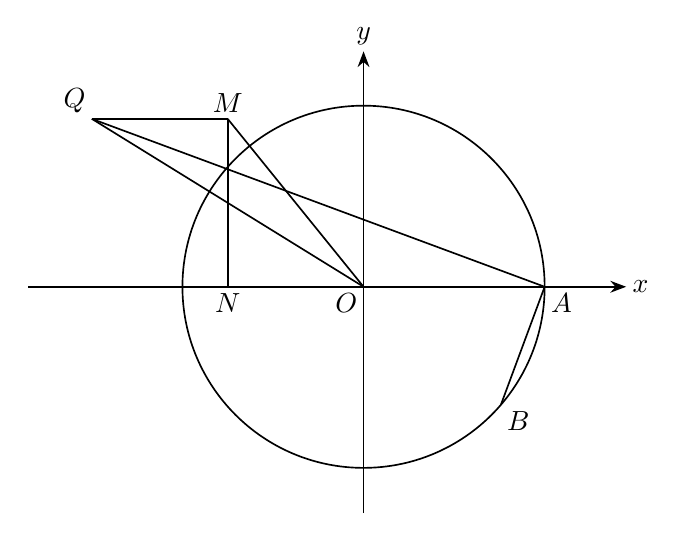
\begin{tikzpicture}[x=1cm,y=1cm,scale=2.3,line width=.6pt,>=Stealth]
\coordinate (O) at (0,0);
\coordinate (A) at (1,0);
\coordinate (M) at (-0.75,0.9270248);
\coordinate (N) at (-0.75,0);
\coordinate (Q) at (-1.5,0.9270248);
\coordinate (B) at (0.7582418,-0.6519735);
\draw (O) circle [radius=1cm];
\draw[->] (-1.85,0)--(1.45,0) node[right,inner sep=0pt,xshift=2pt] {$x$};
\draw[->] (0,-1.25)--(0,1.3) node[above,inner sep=0pt,yshift=2pt] {$y$};
\draw (Q)--(M);
\draw (M)--(N);
\draw (Q)--(O);
\draw (M)--(O);
\draw (Q)--(A);
\draw (A)--(B);
\node[below left,inner sep=2pt] at (O) {$O$};
\node[above left,inner sep=2pt] at (Q) {$Q$};
\node[above,inner sep=2pt] at (M) {$M$};
\node[below,inner sep=2pt] at (N) {$N$};
\node[below right,inner sep=2pt] at (A) {$A$};
\node[below right,inner sep=2pt] at (B) {$B$};
\end{tikzpicture}
